% =====================================================================
%  Tìm kiếm ảnh ký tự Hán-Nôm tương đồng — bản LaTeX định dạng bài hội nghị
%
%  BIÊN DỊCH:  tectonic -X compile report/paper.tex
%          hoặc  latexmk -xelatex -cd report/paper.tex
%
%  BẮT BUỘC dùng XeLaTeX hoặc LuaLaTeX, KHÔNG dùng pdflatex: bài có chữ Nôm nằm
%  ngoài mặt phẳng cơ bản (U+20000..U+2FFFF) nên phải qua fontspec.
%
%  Hình vẽ sinh bằng `make_figures.py` từ số liệu thật; đừng sửa tay file PDF trong figs/.
% =====================================================================
\documentclass[conference,a4paper]{IEEEtran}

\usepackage{fontspec}
\usepackage{graphicx}
\usepackage{booktabs}
\usepackage{amsmath}
\usepackage{amssymb}
\usepackage{array}
\usepackage[hidelinks]{hyperref}
\usepackage{url}

% TeX Gyre Termes = bản Times tự do, phủ đủ dấu tiếng Việt. Gọi theo TÊN FILE chứ không theo tên
% hệ thống ("TeX Gyre Termes"): tên hệ thống cần font được cài vào fontconfig, còn tên file thì mọi
% bản TeX Live / MiKTeX / Tectonic đều tìm được qua kpathsea. Đây là khác biệt giữa "biên dịch được
% trên máy tôi" và "biên dịch được ở mọi nơi".
% Ligatures=TeX để "---" ra gạch dài; CỐ TÌNH không bật cho font mono, nếu không các cờ dòng lệnh
% như --normalize bị nối thành một gạch ngang.
\setmainfont{texgyretermes}[Extension=.otf, UprightFont=*-regular, BoldFont=*-bold,
  ItalicFont=*-italic, BoldItalicFont=*-bolditalic, Ligatures=TeX]
\setsansfont{texgyreheros}[Extension=.otf, UprightFont=*-regular, BoldFont=*-bold,
  ItalicFont=*-italic, BoldItalicFont=*-bolditalic, Ligatures=TeX]
\setmonofont{texgyrecursor}[Extension=.otf, UprightFont=*-regular, BoldFont=*-bold,
  ItalicFont=*-italic, BoldItalicFont=*-bolditalic, Scale=0.86]

% Font chữ Nôm. BabelStone phủ phần lớn; HanaMinB phủ Ext-B (chữ Nôm riêng) mà BabelStone thiếu.
% Đã kiểm bằng bảng cmap: mọi ký tự trong bài đều nằm trong font được gán.
\newfontfamily\nomfont{BabelStoneHan.ttf}[Path=../fonts/]
\newfontfamily\nomfontb{HanaMinB.otf}[Path=../fonts/]
\newcommand{\nom}[1]{{\nomfont #1}}
\newcommand{\nomb}[1]{{\nomfontb #1}}
\newcommand{\code}[1]{{\small\texttt{#1}}}

% Việt hoá các nhãn LaTeX tự sinh. Không đặt thì thân bài ghi "Hình 1" trong khi chú thích ghi
% "Fig. 1" — hai ngôn ngữ trong cùng một tham chiếu.
\renewcommand{\figurename}{Hình}
\renewcommand{\tablename}{Bảng}
\renewcommand{\refname}{Tài liệu tham khảo}
\renewcommand{\appendixname}{Phụ lục}

\begin{document}

\title{Tìm kiếm ảnh ký tự Hán-Nôm tương đồng\\
bằng học tương phản trên cặp dương sinh từ font}

\author{\IEEEauthorblockN{Đồ án môn học}
\IEEEauthorblockA{Mã nguồn, dữ liệu, mô hình và toàn bộ lệnh tái lập kèm theo\\
Trọng số: \url{https://huggingface.co/vohoangkh4ng/chinese-clip-ft-sinonom}}}

\maketitle

\begin{abstract}
Báo cáo trình bày một hệ thống tìm kiếm ảnh ký tự Hán-Nôm tương đồng trên corpus 26.044 glyph, và
quá trình cải thiện nó qua ba bước đo được. Thứ nhất, thay bộ trích đặc trưng ResNet18 của bản gốc
bằng tháp ảnh Chinese-CLIP, nâng \code{radical@k} từ 0,2316 lên 0,5361. Thứ hai, xây dựng phép đánh
giá trên ảnh scan thật thay vì chỉ dựa vào chỉ số proxy: 59 ảnh viết tay có nhãn giải mã từ tên file
và được người đọc kiểm lại; trên tập này mô hình tốt nhất chỉ đạt \code{hit@1} = 0,0847, thấp hơn
hẳn mức mà các chỉ số proxy gợi ý. Thứ ba, fine-tune bằng học tương phản có giám sát trên 141.981
ảnh render đa font với nhãn là mã Unicode, đưa \code{hit@1} trên chính 59 ảnh scan đó lên
\textbf{0,5932} --- hai khoảng tin cậy 95\% rời hẳn nhau. Trên bài toán xếp hạng trong nhóm ký tự
cùng âm Quốc Ngữ, độ chính xác top-1 tăng từ 0,4746 lên \textbf{0,8136}. Các lớp Unicode bị giữ
hoàn toàn ngoài tập huấn luyện đạt kết quả bằng đúng các lớp đã huấn luyện (0,9939 so với 0,9954),
nên phần cải thiện không đến từ ghi nhớ. Chúng tôi cũng khảo sát một tầng xếp hạng lại bằng siêu dữ
liệu ngôn ngữ học và báo cáo nó như một \emph{kết quả âm}: siêu dữ liệu có trần cao (oracle cho
$+17{,}5$ điểm) nhưng suy ra siêu dữ liệu của ảnh truy vấn mới là chỗ nghẽn. Mọi kết quả âm --- kể
cả một lần huấn luyện bị sụp đổ biểu diễn --- được giữ lại vì nguyên nhân của chúng có tính lặp lại.
\end{abstract}

\begin{IEEEkeywords}
truy hồi ảnh, chữ Nôm, học tương phản, SupCon, Chinese-CLIP, xếp hạng lại, kết quả âm
\end{IEEEkeywords}

% =====================================================================
\section{Giới thiệu}

Cho một ảnh glyph Hán-Nôm, bài toán là tìm những ký tự trong corpus có hình dạng gần nó nhất. Hệ
thống được chia làm hai phần ứng với hai tình huống sử dụng khác nhau. \textbf{Phần 1} tìm trên toàn
bộ 26.044 ứng viên khi chưa biết ký tự là gì --- tình huống khó, dùng khi số hoá một trang chữ chưa
được phiên âm. \textbf{Phần 2} xếp hạng trong nhóm ký tự cùng âm Quốc Ngữ khi đã biết chữ đó đọc là
gì, trung vị 7 ứng viên --- tình huống khi hiệu đính một bản phiên âm đã có.

Mục~\ref{sec:related} đặt đồ án vào bối cảnh các công trình đã có.
Đóng góp của báo cáo, theo thứ tự giá trị:

\begin{enumerate}
  \item Một \textbf{phép đánh giá trên dữ liệu thật} thay cho chỉ số proxy: 59 ảnh scan viết tay có
        nhãn, kèm thang tin cậy do người gán độc lập với mọi điểm số của mô hình (mục~\ref{sec:eval}).
  \item \textbf{Fine-tune} (mục~\ref{sec:ft}) nâng \code{hit@1} trên scan thật từ 0,0847 lên
        0,5932, kèm phép kiểm chứng minh kết quả không phải do ghi nhớ (mục~\ref{sec:real},
        \ref{sec:gen}).
  \item Một \textbf{quy trình sinh dữ liệu huấn luyện} từ corpus vốn chỉ có một ảnh mỗi ký tự, bằng
        render đa font cộng mô hình suy giảm ảnh hiệu chỉnh theo số đo của scan thật
        (mục~\ref{sec:render}).
  \item \textbf{Năm kết quả âm} được ghi lại đầy đủ, gồm phân tích trần của chỉ số \code{radical@k},
        một lần sụp đổ biểu diễn khi huấn luyện, và một tầng xếp hạng lại không đạt kỳ vọng
        (mục~\ref{sec:neg}, \ref{sec:rerank}).
\end{enumerate}

% =====================================================================
\section{Công trình liên quan}
\label{sec:related}

\subsection{Biểu diễn ảnh dùng chung}

Truy hồi ảnh hiện đại hầu như luôn bắt đầu từ một backbone đã pretrain rồi mới tính đến việc huấn
luyện riêng. CLIP~\cite{clip} cho thấy một tháp ảnh học từ cặp ảnh--văn bản quy mô web tạo ra không
gian đặc trưng dùng lại được cho nhiều tác vụ mà không cần nhãn của tác vụ đó;
Chinese-CLIP~\cite{chineseclip} lặp lại quy trình ấy trên ngữ liệu tiếng Trung, nên tháp ảnh của nó
đã nhìn thấy chữ Hán trong lúc pretrain --- lý do chúng tôi chọn nó thay vì CLIP gốc.
DINOv2~\cite{dinov2} đại diện cho hướng ngược lại, học hoàn toàn tự giám sát không cần văn bản. Cả
hai đều dùng kiến trúc ViT~\cite{vit}. Baseline của bản gốc là ResNet18~\cite{resnet} pretrain
ImageNet; mục~\ref{sec:neg} cho thấy khoảng cách giữa nó và Chinese-CLIP \emph{không} nằm ở chi tiết
kiến trúc mà mọi người hay đoán.

\subsection{Học metric và học tương phản}

Nhánh học metric có giám sát cổ điển dùng hàm mất mát bộ ba~\cite{facenet}, và điểm mấu chốt trong
thực hành hoá ra không phải công thức mà là \emph{cách lấy mẫu batch}:
Hermans và cộng sự~\cite{intriplet} chỉ ra rằng batch phải được dựng theo lược đồ P lớp $\times$ K
ảnh thì trong batch mới tồn tại cặp dương để so. Đây chính là ràng buộc quyết định ở
mục~\ref{sec:ft}, và bỏ qua nó là nguyên nhân của lần huấn luyện hỏng ở mục~\ref{sec:collapse}.

Nhánh tự giám sát dùng InfoNCE~\cite{infonce} với cặp dương sinh bằng tăng cường ảnh, như trong
SimCLR~\cite{simclr} và MoCo~\cite{moco}. SupCon~\cite{supcon} nối hai nhánh lại: giữ dạng InfoNCE
nhưng lấy \emph{mọi} ảnh cùng nhãn trong batch làm dương. Với bài toán của chúng tôi đây là dạng tự
nhiên nhất --- nhãn (mã Unicode) thì có sẵn và miễn phí, còn số lớp thì quá lớn để đặt một lớp phân
loại lên trên.

Đối lập lại là nhánh softmax có biên góc, tiêu biểu là ArcFace~\cite{arcface}, vốn thống trị nhận
dạng khuôn mặt. Điểm khác biệt thường bị bỏ qua: ArcFace cần một ma trận trọng tâm lớp học được cỡ
$C \times d$. Ở quy mô nhận dạng mặt, mỗi lớp có hàng chục tới hàng trăm ảnh nên ma trận ấy được ước
lượng tốt; ở quy mô của chúng tôi ($C = 23.440$, trung bình 6 ảnh mỗi lớp) thì không.
Mục~\ref{sec:collapse} đo hệ quả. Wang và Isola~\cite{alignuniform} cung cấp đúng công cụ để chẩn
đoán chuyện này: một biểu diễn hỏng vì mất tính \emph{uniformity} trên siêu cầu, và đại lượng đó đo
được rẻ tiền bằng cosine trung bình giữa các cặp ngẫu nhiên --- chỉ số chúng tôi thêm vào vòng đánh
giá sau khi mất một lần huấn luyện vì không có nó.

\subsection{Dữ liệu tổng hợp bằng render}

Khi nhãn thật khan hiếm, render dữ liệu bằng font là một chiến lược đã được kiểm chứng trong nhận
dạng chữ: Jaderberg và cộng sự~\cite{synth90k} huấn luyện bộ nhận dạng chữ cảnh vật hoàn toàn trên
ảnh tổng hợp, và Gupta và cộng sự~\cite{synthtext} mở rộng sang định vị chữ. Cả hai đều nhấn mạnh
rằng ảnh render sạch \emph{một mình} không đủ; phải có một mô hình suy giảm đưa chúng lại gần phân
phối thật. Trong nhận dạng chữ viết tay, biến dạng đàn hồi~\cite{elastic} là ví dụ kinh điển cho ý
tưởng ấy. Đóng góp của chúng tôi ở mục~\ref{sec:render} không phải bản thân ý tưởng mà là việc
\emph{hiệu chỉnh} hàm suy giảm theo số đo lấy trực tiếp từ ảnh scan mục tiêu, thay vì chọn tham số
theo cảm tính, và việc báo cáo khoảng cách còn lại sau khi hiệu chỉnh.

\subsection{Chữ Hán-Nôm}

Chữ Nôm dùng lại kho ký tự Hán cộng thêm các ký tự tự tạo của người Việt, phần lớn nằm trong các khối
CJK Unified Ideographs Extension của Unicode --- trong đó có cả các mặt phẳng ngoài mặt phẳng cơ bản,
điều ràng buộc cả lựa chọn font lẫn cách xử lý chuỗi trong toàn bộ mã nguồn. Tri thức ngôn ngữ học
thường dùng để hỗ trợ tra cứu là bộ thủ, số nét và phân rã IDS (\emph{Ideographic Description
Sequence}) --- đúng ba trường có trong bảng tra của đồ án và là đầu vào cho tầng xếp hạng lại ở
mục~\ref{sec:rerank}. Điểm chúng tôi muốn nhấn: các trường này rất hấp dẫn để dùng làm \emph{chỉ số
đánh giá} vì chúng có sẵn, nhưng mục~\ref{sec:neg} cho thấy chúng là nhãn yếu, và mục~\ref{sec:ft}
giải thích vì sao huấn luyện trên chúng rồi báo cáo chính chúng là một vòng lặp khép kín.

% =====================================================================
\section{Dữ liệu}

\begin{table}[t]
\caption{Các tập dữ liệu. Ba tập đầu là đầu vào cho trước; hai tập sau do nhóm tạo hoặc gán nhãn.}
\label{tab:data}
\centering\small
% Cột p{} mặc định căn đều hai bên, làm chữ giãn xấu trong ô hẹp -> ép raggedright.
\newcolumntype{L}[1]{>{\raggedright\arraybackslash}p{#1}}
\begin{tabular}{@{}L{1.95cm}L{1.75cm}L{3.85cm}@{}}
\toprule
Tập & Kích thước & Vai trò \\
\midrule
\code{images/}      & 26.044 ảnh  & Corpus tra cứu. Mỗi ký tự đúng \textbf{một} ảnh. \\
\code{final\_...}    & 31.208 dòng & Bộ thủ, số nét, phân rã IDS. \\
\code{QuocNgu...}   & ---         & Ánh xạ âm Quốc Ngữ $\leftrightarrow$ ký tự. \\
\code{test\_images/} & 59 ảnh scan & \textbf{Tập đánh giá thật} (viết tay). \\
\code{rendered/}    & 131.604 ảnh & Sinh ra để huấn luyện, qua 7 font. \\
\bottomrule
\end{tabular}
\end{table}

Bảng~\ref{tab:data} liệt kê các tập dữ liệu. Đặc điểm quyết định toàn bộ thiết kế:
\textbf{corpus chỉ có một ảnh cho mỗi ký tự}. Học metric cần
cặp dương --- hai ảnh khác nhau của cùng một lớp --- nên trong dữ liệu gốc \emph{không tồn tại cặp
nào}. Mục~\ref{sec:render} giải quyết đúng chỗ này.

Ảnh trong \code{test\_images/} được đặt tên bằng kiểu gõ Telex (\code{cofn.jpg} = ``còn''), nên giải
mã ngược ra chữ Quốc Ngữ rồi tra từ điển sẽ được \textbf{tập ký tự đúng} cho ảnh đó. Đây là nhãn
thật, không phải proxy, và là lý do tập 59 ảnh này có giá trị lớn hơn nhiều so với kích thước của nó.

% =====================================================================
\section{Phương pháp}

\subsection{Trích đặc trưng và tìm kiếm}

Mọi backend đưa ảnh về một vector đã chuẩn hoá L2 nên tích vô hướng chính là cosine. Tìm kiếm dùng
Faiss \code{IndexFlatIP}~\cite{faiss} --- tìm chính xác, không xấp xỉ. Bản gốc dùng ResNet18~\cite{resnet}
pretrain ImageNet với lớp \code{conv1} thay bằng lớp 1 kênh khởi tạo ngẫu nhiên; chúng tôi giữ bản
này nguyên vẹn từng bit làm mốc ``trước'', và thêm năm backend để so, gồm ba cỡ
Chinese-CLIP~\cite{chineseclip} và DINOv2~\cite{dinov2}.

\subsection{Sinh cặp dương bằng render đa font}
\label{sec:render}

Vì mỗi ký tự chỉ có một ảnh, chúng tôi render lại từng mã Unicode qua bảy font Hán-Nôm khác nhau:
cùng một lớp, khác kiểu chữ. Độ phủ được kiểm bằng bảng \code{cmap} của từng font chứ không phỏng
đoán; hợp nhất lại phủ 26.033/26.044 ký tự. \textbf{Ký tự không có trong \code{cmap} bị bỏ qua},
vì nếu render bừa thì font trả về ô tofu --- một ô vuông rỗng giống hệt nhau ở mọi ký tự --- đưa vào
huấn luyện sẽ đầu độc cặp dương.

Nhưng tập render sạch \emph{quá dễ}: ảnh render tự truy hồi đúng chữ ở \code{hit@1} = 0,7018 trong
khi scan thật chỉ đạt 0,0847, chênh gần chín lần. Nghĩa là phần lớn khoảng cách tới thực tế không
nằm ở font. Chúng tôi đo sáu chỉ số ảnh trên hai tập để tìm chỗ lệch (Bảng~\ref{tab:degrade}) rồi
xây hàm \code{degrade()} mô phỏng đúng sáu trục đó theo thứ tự vật lý của một trang scan. Mọi phép
biến đổi đều là nhiễu ảnh, \emph{không đụng tới cấu trúc bộ thủ}, nên nhãn vẫn đúng. Kết quả:
\code{hit@1} của tập render tụt từ 0,7018 xuống 0,1986 --- chỉ còn dễ hơn scan thật 2,8 lần thay vì
9 lần.

\begin{table}[t]
\caption{Khoảng cách đo được giữa scan thật và ảnh render. Hàm suy giảm mô phỏng đúng sáu trục này.}
\label{tab:degrade}
\centering\small
\begin{tabular}{@{}lrrrl@{}}
\toprule
Chỉ số & Scan & Render & Tỉ lệ & Ý nghĩa \\
\midrule
edge     & 15,6 & 102,3 & 0,15$\times$ & scan mờ hơn nhiều \\
contrast & 91,6 & 232,8 & 0,39$\times$ & mực xám nhạt \\
thick    & 0,051 & 0,028 & 1,82$\times$ & nét scan dày gấp đôi \\
fill     & 0,349 & 0,206 & 1,69$\times$ & hệ quả của nét dày \\
noise    & 10,1 & 2,7   & 3,77$\times$ & hạt nhiễu giấy \\
bg       & 254,0 & 255,0 & $\approx$1$\times$ & nền giấy hơi ngà \\
\bottomrule
\end{tabular}
\end{table}

Phần 2,8 lần còn lại là khác biệt \textbf{cấu trúc} (bút lông, lối hành thư: nét nối liền, tỉ lệ bộ
phận xê dịch, có nét bị lược) và không thể sinh ra từ một ảnh in bằng xử lý ảnh.

\subsection{Fine-tune}
\label{sec:ft}

Mục tiêu học là \textbf{bất biến kiểu chữ}: cùng một mã Unicode qua font khác nhau phải cho cùng một
vector. Nhãn duy nhất là mã Unicode --- cố ý \emph{không} dùng \code{RADICAL} hay \code{STROKE\_NUM},
vì huấn luyện trên một nhãn ngôn ngữ học rồi báo cáo chính chỉ số của nhãn đó là đo lại tập huấn
luyện chứ không phải đánh giá.

\begin{table}[t]
\caption{Cấu hình fine-tune.}
\label{tab:ft}
\centering\small
\begin{tabular}{@{}p{1.6cm}p{6.0cm}@{}}
\toprule
Thành phần & Lựa chọn \\
\midrule
Backbone & Chinese-CLIP ViT-B/16, giữ nguyên \code{visual\_projection} (512 chiều) \\
Hàm mất mát & SupCon~\cite{supcon}, nhiệt độ 0,07 \\
Lấy mẫu & \textbf{P$\times$K: 24 lớp $\times$ 2 view mỗi batch} \\
Dữ liệu & 141.981 ảnh / 23.440 lớp \\
Suy giảm & \code{degrade()} chạy \textbf{trực tuyến} trong DataLoader, $p = 0{,}6$ \\
Tối ưu & AdamW, lr $10^{-5}$, warmup 300, cosine, bf16 \\
Chi phí & \textbf{3,7\,GB VRAM}, $\sim$4 phút/epoch, 6 epoch \\
\bottomrule
\end{tabular}
\end{table}

Công thức hàm mất mát và lược đồ lấy mẫu được viết đầy đủ ở mục~\ref{sec:loss}.
Hai lựa chọn trong Bảng~\ref{tab:ft} là \textbf{điều kiện sống còn chứ không phải tinh chỉnh}, và cả
hai đều đến từ lần thất bại ở mục~\ref{sec:collapse}:

\begin{itemize}
  \item \textbf{Lấy mẫu P$\times$K.} Một batch 48 ảnh rút ngẫu nhiên từ 23.440 lớp chỉ chứa khoảng
        0,05 cặp dương theo kỳ vọng --- gần như mọi batch sẽ không có gì để kéo lại gần nhau, và hàm
        mất mát trở thành hằng số.
  \item \textbf{SupCon thay vì softmax có biên góc.} SupCon không có tham số học được nào trong hàm
        mất mát, nên không có một head khởi tạo ngẫu nhiên bơm nhiễu ngược về backbone.
\end{itemize}

Suy giảm ảnh chạy \emph{trực tuyến lúc nạp dữ liệu} chứ không render sẵn ra đĩa: bộ sinh số ngẫu
nhiên gieo theo bộ ba (seed, epoch, chỉ số ảnh) nên mỗi epoch mỗi ảnh có một biến thể khác, vẫn tái
lập được, và không tốn thêm dung lượng nào.

\subsection{Hàm mất mát và lược đồ lấy mẫu, viết đầy đủ}
\label{sec:loss}

Gọi $B$ là batch, $z_i = f_\theta(x_i)/\lVert f_\theta(x_i)\rVert_2$ là embedding đã chuẩn hoá,
$y_i$ là mã Unicode của ảnh $x_i$, và $\tau = 0{,}07$. Đặt $P(i) = \{p \in B : y_p = y_i,\, p \neq
i\}$ là tập dương của neo $i$. Hàm mất mát SupCon~\cite{supcon} là

\begin{equation}
\label{eq:supcon}
\mathcal{L} = \frac{1}{|A|}\sum_{i \in A}
\frac{-1}{|P(i)|}\sum_{p \in P(i)}
\log \frac{\exp(z_i^{\!\top} z_p/\tau)}
          {\displaystyle\sum_{a \in B \setminus \{i\}} \exp(z_i^{\!\top} z_a/\tau)},
\end{equation}

trong đó $A = \{i \in B : |P(i)| > 0\}$. Ba chi tiết cài đặt không đọc ra được từ~\eqref{eq:supcon}
nhưng quyết định việc nó có chạy hay không:

\begin{enumerate}
  \item \textbf{Mẫu số bỏ chính neo}, nên đường chéo của ma trận tương đồng phải bị che. Cách che
        chuẩn là gán $-\infty$ trước khi lấy \code{logsumexp}.
  \item \textbf{$-\infty \cdot 0 = \mathrm{NaN}$ theo IEEE 754.} Sau \code{logsumexp}, đường chéo
        vẫn còn $-\infty$; nhân nó với mặt nạ dương (giá trị 0 tại đường chéo) cho NaN, và toàn bộ
        gradient thành NaN ngay bước đầu tiên. Phải \emph{gán lại đường chéo về 0} sau
        \code{logsumexp} và trước phép nhân mặt nạ. Đây là lỗi chúng tôi thực sự gặp.
  \item \textbf{Neo không có dương phải bị loại khỏi trung bình}, không phải cho bằng 0: gộp chúng
        vào làm hàm mất mát bị chia nhỏ tuỳ theo có bao nhiêu lớp lẻ trong batch.
\end{enumerate}

Giá trị của~\eqref{eq:supcon} khi biểu diễn sụp đổ hoàn toàn (mọi $z_i$ trùng nhau) là
$\ln(PK - 1) = \ln 47 \approx 3{,}85$; con số này là \emph{dấu hiệu chẩn đoán} chứ không phải một
mức mất mát ngẫu nhiên, và biết nó cho phép phát hiện sụp đổ chỉ bằng cách nhìn hàm mất mát.

\medskip
Lược đồ lấy mẫu được viết thành một \code{Sampler} riêng thay vì trộn ngẫu nhiên:

{\footnotesize\ttfamily\raggedright
\textbf{Thuật toán 1: PKSampler}(nhãn, batch$=48$, K$=2$)\\
1\ \ P $\leftarrow$ max(2, batch // K)\ \ \ \ \# 24 lớp mỗi batch\\
2\ \ bỏ mọi lớp có $<$ K ảnh\ \ \ \ \ \ \ \# không dựng nổi cặp dương\\
3\ \ lặp mỗi epoch:\\
4\ \ \ \ \ hoán vị ngẫu nhiên danh sách lớp\\
5\ \ \ \ \ với mỗi khối P lớp liên tiếp:\\
6\ \ \ \ \ \ \ \ với mỗi lớp trong khối:\\
7\ \ \ \ \ \ \ \ \ \ \ lấy K ảnh, không lặp trong epoch\\
8\ \ \ \ \ \ \ \ trả về P$\cdot$K chỉ số làm một batch\\
}

\medskip
Vì sao bước 1--2 là bắt buộc chứ không phải tinh chỉnh: với $C = 23.440$ lớp và batch ngẫu nhiên cỡ
$B = 48$, số cặp dương kỳ vọng trong batch là

\begin{equation}
\label{eq:pairs}
\mathbb{E}[\#\text{cặp dương}] = \binom{B}{2}\Pr[y_i{=}y_j] \approx 1128 \cdot \frac{1}{23.440}
\;\approx\; 0{,}05 .
\end{equation}

Tức là \textbf{khoảng 95\% số batch hoàn toàn không có gì để kéo lại gần nhau}, và với những batch
đó~\eqref{eq:supcon} không có số hạng nào --- hàm mất mát trở thành hằng số và gradient bằng không.
Không có công thức mất mát nào cứu được chuyện này; nó là lỗi ở tầng lấy mẫu.

% =====================================================================
\section{Phương pháp đánh giá}
\label{sec:eval}

Phần lớn công sức của đồ án nằm ở chỗ này, vì một chỉ số sai làm mọi kết luận phía sau vô nghĩa. Ba
tầng đánh giá, xếp theo độ tin cậy tăng dần: \emph{chỉ số proxy} trên toàn corpus (\code{radical@k},
\code{stroke\_mae@k}, \code{ids\_jaccard@k}) --- rẻ nhưng là nhãn yếu; \emph{nhãn thật từ tên file}
trên 59 ảnh scan, với mức ngẫu nhiên khoảng $4{,}7\cdot10^{-4}$; và \emph{nhãn do người gán} cho
Phần 2, đã gán đủ 59/59 ảnh.

Cột \code{confidence} trong bảng nhãn là \textbf{đánh giá của người đọc ảnh, không suy ra từ bất kỳ
điểm số nào của mô hình.} Điều này là cố ý: phép kiểm độ nhạy dùng chính cột này để lọc ra tập nhãn
chắc chắn rồi chấm lại mô hình trên đó, nên nếu \code{confidence} lấy từ điểm similarity thì phép
kiểm ấy thành vòng tròn --- lấy mô hình chấm mô hình. Thang gồm ba mức \emph{high} (nét quyết định
đọc được), \emph{med} (còn ít nhất một biến thể gần trùng chỉ khác ở chi tiết đã mờ) và \emph{low}
(lựa chọn dựa vào văn cảnh nhiều hơn hình), phân bố cuối cùng 53/4/2.

Các ảnh scan là những dòng mở đầu \emph{Truyện Kiều}, nên nhãn được gán bằng so hình trước rồi đối
chiếu với chính tả Nôm chuẩn của tác phẩm. \textbf{Khi hình và văn cảnh mâu thuẫn thì hình thắng},
và \code{confidence} bị hạ xuống \emph{med} --- bản scan viết ``qua'' là \nom{戈} chứ không phải
\nom{過}, ``năm'' là \nom{𢆥} chứ không phải \nom{年}.

\subsection{Định nghĩa chỉ số}

Để tránh mơ hồ, các chỉ số được viết ra đầy đủ. Với $N$ truy vấn, gọi $r_q$ là thứ hạng (bắt đầu từ
1) của ứng viên đúng đầu tiên cho truy vấn $q$; nếu không có ứng viên đúng nào trong danh sách trả
về thì $1/r_q \mathrel{:}= 0$.

\begin{align}
\text{hit@}k &= \frac{1}{N}\sum_{q=1}^{N} \mathbf{1}[\,r_q \leq k\,],
& \text{MRR} &= \frac{1}{N}\sum_{q=1}^{N} \frac{1}{r_q}.
\end{align}

\code{radical@k} là chỉ số \emph{proxy}: tỉ lệ trong $k$ ứng viên đầu có cùng bộ thủ với truy vấn,
lấy trung bình trên mọi truy vấn. Nó không cần nhãn thật, đó vừa là ưu điểm (chạy được trên cả
26.044 ký tự) vừa là nhược điểm --- mục~\ref{sec:neg} đo trần của chính nó.

Khoảng tin cậy dùng công thức Wilson~\cite{wilson} chứ không dùng xấp xỉ chuẩn (Wald). Với $\hat{p}$
là tỉ lệ quan sát, $n$ là cỡ mẫu và $z = 1{,}96$:

\begin{equation}
\label{eq:wilson}
\frac{\hat{p} + \dfrac{z^2}{2n} \pm z\sqrt{\dfrac{\hat{p}(1-\hat{p})}{n} + \dfrac{z^2}{4n^2}}}
     {1 + \dfrac{z^2}{n}} .
\end{equation}

Lý do: ở $n = 59$ và các tỉ lệ gần 0 mà chúng tôi thực sự đo được ở cấu hình zero-shot
($\hat{p} = 0{,}0847$), khoảng Wald tràn qua 0 và cho cận dưới âm --- một khoảng tin cậy vô nghĩa
cho một tỉ lệ. Wilson không bao giờ ra ngoài $[0,1]$.

\textbf{Mọi tỉ lệ đều kèm khoảng tin cậy nhị thức 95\%}~\cite{wilson}. Với $n = 59$ và $p \approx
0{,}5$, khoảng tin cậy rộng khoảng $\pm13$ điểm, nên bất kỳ cải thiện nào dưới $\sim$15 điểm đều
không chứng minh được. Đây là giới hạn cứng của tập test hiện có, và báo cáo tuân thủ nó một cách
nhất quán: trong toàn bộ đồ án chỉ có đúng một so sánh vượt qua được ngưỡng này.

% =====================================================================
\section{Kết quả}

\subsection{So sánh backend trên toàn corpus}

\begin{table}[t]
\caption{Toàn bộ corpus 26.044 glyph, top-$K$ = 20. Đậm là tốt nhất mỗi cột.}
\label{tab:backend}
\centering\footnotesize
\begin{tabular}{@{}lrrrr@{}}
\toprule
Backend & radical@k $\uparrow$ & stroke $\downarrow$ & ids @k $\uparrow$ & img/s \\
\midrule
\code{resnet18} (gốc)      & 0,2316 & 2,8942 & 0,1031 & \textbf{3950} \\
\code{resnet18-gray}       & 0,2202 & 2,5658 & 0,1020 & 3937 \\
\code{chinese-clip} B/16   & 0,4843 & 2,6296 & 0,1997 & 358 \\
\code{chinese-clip-large}  & \textbf{0,5361} & 2,6992 & 0,2113 & 354 \\
\code{chinese-clip-huge}   & 0,5147 & 2,6547 & \textbf{0,2144} & 283 \\
\code{dinov2}              & 0,3081 & \textbf{2,3397} & 0,1251 & 306 \\
\bottomrule
\end{tabular}
\end{table}

Bảng~\ref{tab:backend} cho kết quả. Chinese-CLIP thắng với biên độ lớn: \code{radical@k} gấp \textbf{2,31 lần} bản gốc và
\code{ids\_jaccard} gấp 2,05 lần, mà gần như không tốn thêm thời gian (354 so với 358 ảnh/giây).
DINOv2 thua ở bộ thủ nhưng \emph{thắng ở số nét}, và chỉ trùng 12,9\% kết quả top-$k$ với họ CLIP,
nên nó không đơn thuần là kém hơn mà mạnh ở một trục khác.

\subsection{Trần của chính chỉ số proxy}

Một câu hỏi được đặt ra: \code{radical@k} $\approx 0{,}5$ có phải đã bão hoà? Giả thuyết ``tập
top-$k$ thiếu ứng viên đúng'' \textbf{bị bác bỏ}: trần lý thuyết của \code{radical@20} là 0,9862,
tức chỉ 3\% query bị chạm trần; và \code{radical@1} cũng chỉ đạt 0,6331, nên chỗ nghẽn nằm ngay ở
láng giềng gần nhất chứ không ở đuôi danh sách.

Nhưng phép kiểm làm lộ ra một điều quan trọng hơn: \textbf{\code{RADICAL} không phải nhãn thị giác
thuần tuý.} Bộ thủ chỉ thực sự xuất hiện trong hình chữ ở 56,7\% số ký tự; phần còn lại mang bộ thủ
vì lý do từ nguyên hoặc quy ước tra cứu, không phải vì trông giống. Một oracle \emph{biết trước}
phân rã IDS cũng chỉ đạt \code{radical@20} = 0,7338. So với trần thực tế đó, \code{chinese-clip-large}
(0,5361) đang ở \textbf{73\% quãng đường} và 24,4 lần mức ngẫu nhiên. Kết luận: chưa bão hoà, nhưng
cũng không nên tiếp tục tối ưu cho một chỉ số mà bản thân nó chỉ đúng ở hai phần ba.

\subsection{Kết quả trên ảnh scan thật}
\label{sec:real}

\begin{figure}[t]
\centering
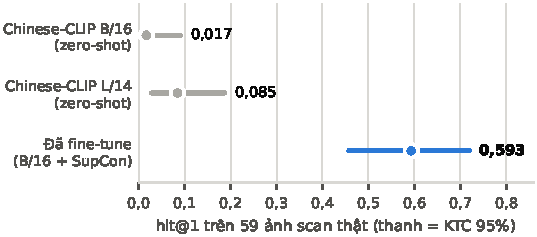
\includegraphics[width=\columnwidth]{figs/fig1-headline.pdf}
\caption{Kết quả chính. \code{hit@1} khi tìm trên toàn bộ 26.044 ký tự, đo trên 59 ảnh scan thật.
Thanh ngang là khoảng tin cậy nhị thức 95\%. \textbf{Hai khoảng của bản zero-shot và bản fine-tune
rời hẳn nhau} --- đây là so sánh duy nhất trong đồ án mà $n = 59$ đỡ nổi một kết luận.}
\label{fig:headline}
\end{figure}

Đây là phép đo duy nhất không phải proxy, và là con số nên dùng để đánh giá đồ án. Không một pixel
nào của \code{test\_images/} đi vào huấn luyện; điều này được bảo đảm bằng một \code{assert} chạy
trước mỗi lần huấn luyện chứ không bằng quy ước.

Hình~\ref{fig:headline} cho thấy khoảng cách. Bản fine-tune đạt \code{hit@1} = 0,5932
$[0{,}457; 0{,}719]$ so với 0,0847 $[0{,}028; 0{,}187]$ của \code{chinese-clip-large} zero-shot ---
35/59 so với 5/59, hơn mức ngẫu nhiên 1.250 lần. \code{hit@10} là 0,7966 và MRR là 0,6691.

Trước fine-tune, kết quả thấp \textbf{không phải vì mô hình kém mà vì lệch phân phối}. Triệu chứng
là hiệu ứng hub: ký tự \nom{攅} được trả về ở vị trí một cho sáu query khác nhau. Query là chữ viết
tay lối hành thư, corpus là khải thư in bằng font. Chúng tôi đã thử chuẩn hoá hình học (cắt sát nét
mực, đệm vào khung vuông) và kết quả nằm trong khoảng nhiễu --- phần lệch hình học có thật nhưng
không phải nguyên nhân chính.

\begin{table}[t]
\caption{Phần 2 --- xếp hạng trong nhóm cùng âm Quốc Ngữ, $n = 59$.}
\label{tab:part2}
\centering\footnotesize
\begin{tabular}{@{}lrrl@{}}
\toprule
Phương pháp & Đúng top-1 & MRR & KTC 95\% \\
\midrule
Chọn ngẫu nhiên trong nhóm & 0,1987 & --- & --- \\
\code{histogram} (bản gốc) & 0,4407 & 0,6070 & [0,312; 0,576] \\
\code{embedding} zero-shot & 0,4746 & 0,6566 & [0,343; 0,609] \\
\textbf{\code{embedding} fine-tune} & \textbf{0,8136} & \textbf{0,8983} & \textbf{[0,691; 0,903]} \\
\bottomrule
\end{tabular}
\end{table}

Bảng~\ref{tab:part2} cho Phần 2. Phép thử độ nhạy trên 53 nhãn \emph{high} cho 0,8491 so với
histogram 0,4717, nên kết luận không phụ thuộc vào sáu nhãn \emph{med}/\emph{low} còn lại.

Bảng này \textbf{sửa lại một kết luận trước đó của chính nhóm}. Với mô hình zero-shot, khoảng cách
giữa embedding và histogram chỉ là \emph{hai ảnh trên 59} --- nằm gọn trong nhiễu --- nên khuyến
nghị dùng embedding khi ấy phải dựa vào chất lượng điểm số chứ không dám viện độ chính xác. Sau
fine-tune, khoảng cách là 22 ảnh và hai khoảng tin cậy rời nhau: độ chính xác đã đủ để tự đứng làm
lý do.

\subsection{Có phải mô hình chỉ ghi nhớ 23.440 danh tính?}
\label{sec:gen}

\begin{figure}[t]
\centering
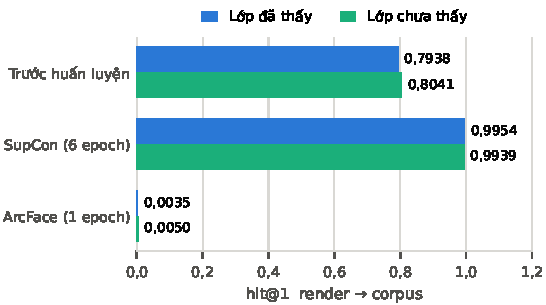
\includegraphics[width=\columnwidth]{figs/fig3-generalisation.pdf}
\caption{Phép kiểm tổng quát hoá. 2.604 mã Unicode bị gỡ \emph{toàn bộ view} khỏi tập huấn luyện ---
chia theo \emph{lớp} chứ không theo ảnh. Sau SupCon, lớp chưa thấy đạt bằng lớp đã thấy. ArcFace sụp
ở \emph{cả hai}, dấu hiệu của sụp đổ biểu diễn chứ không phải overfit.}
\label{fig:gen}
\end{figure}

Đây là phản biện hiển nhiên nhất với một kết quả tăng mạnh như vậy, nên chúng tôi thiết kế phép kiểm
cho nó ngay từ đầu. Chia theo lớp chứ không theo ảnh, vì chia theo ảnh thì lớp nào cũng có mặt ở cả
hai bên và phép đo mất sạch ý nghĩa. Hai mẫu cùng cỡ 2.604 và cùng cách chọn ngẫu nhiên --- chọn
theo thứ tự mã Unicode sẽ thiên về khối CJK cơ bản trong khi held-out rải đều cả Ext-B.

Hình~\ref{fig:gen} cho kết quả: 0,9954 so với \textbf{0,9939}. Bằng nhau. Điều này khớp với cơ chế:
SupCon không có tâm lớp học được nên không có gì để ghi nhớ --- thứ nó học là \emph{phép so hai ảnh},
và phép đó chuyển sang ký tự chưa từng gặp nguyên vẹn.

\subsection{Quan sát định tính}

\begin{figure}[t]
\centering
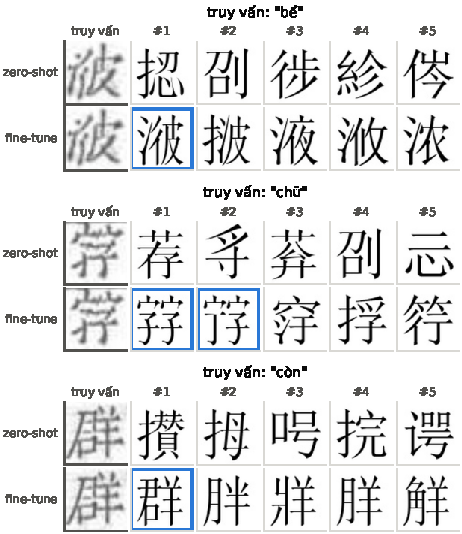
\includegraphics[width=\columnwidth]{figs/fig5-qualitative.pdf}
\caption{Năm láng giềng đầu cho ba ảnh scan thật, trước và sau fine-tune. Khung xanh = ký tự đúng.
Truy vấn được chọn theo quy tắc cố định --- những ảnh mà bản fine-tune đúng ở hạng 1 còn zero-shot
sai ở hạng 1, lấy theo thứ tự tên file --- chứ không bới tìm ví dụ đẹp. Bản zero-shot trả về các ký
tự không liên quan về cấu trúc; bản fine-tune trả về đúng chữ và các biến thể cùng bộ.}
\label{fig:qual}
\end{figure}

Hình~\ref{fig:qual} cho thấy mô hình \emph{làm gì} chứ không chỉ ghi được bao nhiêu điểm. Đáng chú ý
ở truy vấn ``chữ'': bản fine-tune trả về hai biến thể đúng ở hai vị trí đầu, đều mang thành phần
\nom{字}, trong khi bản zero-shot trả về những chữ chỉ giống ở mật độ nét.

% =====================================================================
\section{Kết quả âm}
\label{sec:neg}

Bốn kết quả dưới đây đều là thất bại hoặc bác bỏ, và đều được giữ lại vì chúng loại trừ được những
hướng mà người đọc báo cáo này rất dễ thử lại.

\subsection{Giả thuyết ``lỗi nằm ở \code{conv1}'' --- sai}

Bản gốc thay \code{conv1} bằng lớp 1 kênh khởi tạo ngẫu nhiên, tức vứt bỏ bộ lọc tầng đầu đã
pretrain. Giả thuyết tự nhiên là chỉ cần vá dòng đó. Chúng tôi dựng \code{resnet18-gray} gieo
\code{conv1} bằng tổng các bộ lọc RGB pretrain --- kết quả \code{radical@k} \textbf{giảm nhẹ}
(0,2202 so với 0,2316). Sửa một dòng không cứu được kiến trúc; đây chính là bằng chứng biện minh cho
việc đổi hẳn sang ViT thay vì vá baseline.

\subsection{Scale có lợi, rồi đảo chiều}

base $\rightarrow$ large là $+10{,}7\%$ tương đối trên \code{radical@k}, nhưng large $\rightarrow$
huge là \textbf{$-4{,}0\%$} trong khi tốn thêm 33\% số chiều và 20\% thời gian. Đường cong đã quay
đầu. Đây là chữ ký của ``thêm dung lượng cho một mục tiêu huấn luyện sai domain'' --- và cũng chính
là lý do khiến fine-tune trở thành hướng đáng làm nhất, thay vì đổi sang checkpoint lớn hơn.

\subsection{ArcFace gây sụp đổ biểu diễn}
\label{sec:collapse}

\begin{figure}[t]
\centering
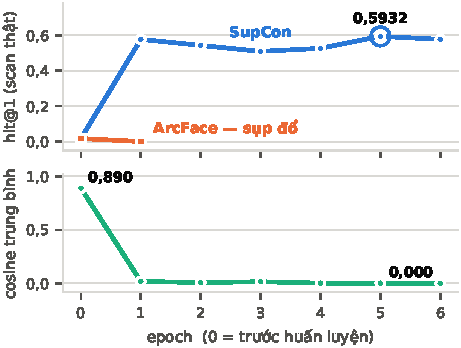
\includegraphics[width=\columnwidth]{figs/fig2-training.pdf}
\caption{Động lực huấn luyện. \emph{Trên}: \code{hit@1} trên scan thật qua từng epoch; ArcFace mất
toàn bộ khả năng truy hồi sau một epoch. \emph{Dưới}: cosine trung bình giữa 2.000 vector corpus
ngẫu nhiên --- máy dò sụp đổ. Con số 0,890 lúc zero-shot tự nó giải thích vì sao khả năng phân biệt
trước đây yếu; sau huấn luyện không gian giãn ra gần trực giao. Hai đại lượng khác thang nên vẽ ở
hai bảng riêng, không dùng hai trục $y$ chồng nhau.}
\label{fig:train}
\end{figure}

Thiết kế fine-tune đầu tiên dùng ArcFace~\cite{arcface} trên 23.440 lớp (scale 32, biên 0,30). Sau
một epoch, \code{hit@1} trên scan thật về 0 và truy hồi render$\rightarrow$corpus rơi từ 0,79 xuống
0,0035 trên lớp đã thấy và 0,80 xuống 0,0050 trên lớp chưa thấy (Hình~\ref{fig:gen},
Hình~\ref{fig:train}).

Sụp ở \emph{cả hai} phía nên đây không phải overfit mà là \textbf{sụp đổ biểu diễn}: mọi ảnh dồn về
một vector. Nguyên nhân nằm ở hình dạng dữ liệu chứ không phải siêu tham số --- 23.440 lớp mà mỗi lớp
chỉ khoảng 6 ảnh. Head ArcFace khởi tạo ngẫu nhiên với 23.440 tâm không bao giờ kịp tổ chức, nên thứ
nó truyền ngược về backbone gần như là nhiễu. Và vì Adam chuẩn hoá theo độ lớn gradient, ``tốc độ
học nhỏ'' $10^{-5}$ vẫn dịch chuyển trọng số đủ để phá cấu trúc pretrain trong khoảng 3.000 bước;
cắt chuẩn gradient không cứu được, vì nhiễu bị cắt chuẩn vẫn là nhiễu.

Ba công cụ chẩn đoán được thêm vào sau lần này, và nên có trong bất kỳ thí nghiệm tương tự nào:
(a) đánh giá \emph{giữa epoch} để sự cố lộ ra sau một phút thay vì sau một giờ; (b) cột đo
\textbf{cosine trung bình} ở Hình~\ref{fig:train} --- nó chạy về 1,0 khi sụp đổ, và nếu không có nó
thì ``học hỏng'' với ``sụp đổ'' trông giống hệt nhau trên \code{hit@1} trong khi hai thứ đó phải sửa
theo hai cách khác nhau; (c) biết trước chữ ký sụp đổ của SupCon là hàm mất mát đứng đúng ở
$\ln(P\!\cdot\!K - 1)$.

\subsection{Một nhãn sai đã tự làm giảm kết quả của chính nhóm}

\begin{figure}[t]
\centering
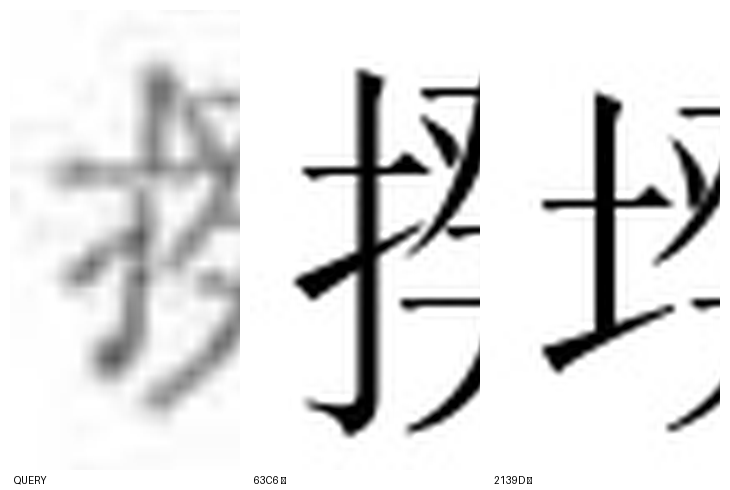
\includegraphics[width=0.62\columnwidth]{figs/coix-bo-trai.png}
\caption{Bộ bên trái của một ảnh scan, phóng to. Nét dọc \emph{dừng} ở vạch ngang nên đây là
\nom{土} chứ không phải \nom{扌} (móc kéo xuống dưới vạch). Sửa nhãn này làm khoảng cách giữa hai
phương pháp co từ bốn ảnh xuống hai --- tức đi ngược lợi ích của kết luận nhóm đang muốn chứng minh.}
\label{fig:coix}
\end{figure}

Khi soát lại 11 dòng \emph{med}/\emph{low}, chúng tôi phát hiện một nhãn gán sai
(Hình~\ref{fig:coix}). Ghi lại điều này vì nó là thước đo trực tiếp cho việc một bảng số ở $n = 59$
nhạy tới mức nào với đúng một nhãn.

% =====================================================================
\section{Xếp hạng lại bằng siêu dữ liệu}
\label{sec:rerank}

Ba cột siêu dữ liệu ngôn ngữ học (\code{RADICAL}, \code{STROKE\_NUM}, \code{SHAPE\_MORPH}) mô tả
những thuộc tính mà mô hình ảnh không nhìn thấy. Câu hỏi tự nhiên: dùng chúng để \textbf{xếp hạng
lại} danh sách ứng viên mà tầng ảnh trả về thì có tốt hơn không? Câu trả lời là \emph{chưa}, và lý
do cụ thể hơn nhiều so với ``không hiệu quả''.

\begin{figure}[t]
\centering
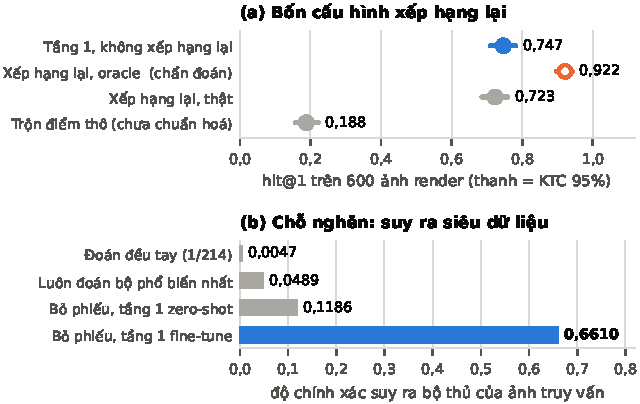
\includegraphics[width=\columnwidth]{figs/fig4-rerank.pdf}
\caption{(a) Bốn cấu hình xếp hạng lại trên 600 ảnh render, tầng 1 là \code{chinese-clip-large}.
Cấu hình oracle vẽ rỗng ruột vì nó \emph{cố tình} đọc trộm siêu dữ liệu thật của truy vấn --- một
chẩn đoán, không phải kết quả. (b) Chỗ nghẽn đã định lượng: độ chính xác suy ra bộ thủ của ảnh truy
vấn, so với hai mốc đoán mò.}
\label{fig:rerank}
\end{figure}

\subsection{Vì sao không thể chấm bằng chỉ số cũ}

Ba chỉ số proxy được suy ra từ \emph{đúng ba cột} mà tầng xếp hạng lại dùng làm đặc trưng. Chấm nó
bằng \code{radical@k} là vòng tròn: điểm số sẽ leo về trần 0,978 mà không chứng minh được gì, vì mô
hình được đưa sẵn đáp án. Phép đo trung thực phải dùng nhãn \textbf{độc lập} với ba cột đó --- ở đây
là mã Unicode của chính ký tự, trên tập ảnh render ($n = 600$, khoảng tin cậy $\pm3{,}5$ điểm).

\subsection{Ba điều rút ra}

Từ Hình~\ref{fig:rerank}(a), theo thứ tự quan trọng:

\begin{itemize}
  \item \textbf{Chuẩn hoá tín hiệu trước khi trộn là bắt buộc.} Trộn điểm thô làm mất 56 điểm
        \code{hit@1} (0,7467 $\rightarrow$ 0,1883). Lý do: với trọng số mặc định, một ứng viên phải
        thắng về độ giống ảnh hơn 0,364 cosine mới bù nổi một lần lệch bộ thủ, mà khoảng cách cosine
        trong top-20 không bao giờ rộng đến thế. Trộn thô vì vậy biến phép xếp hạng thành
        \textbf{sắp xếp từ điển} --- bộ thủ trước, rồi số nét --- đẩy mô hình ảnh xuống làm tiêu chí
        phá hoà.
  \item \textbf{Siêu dữ liệu có trần cao.} Cấu hình oracle được $+17{,}5$ điểm. Vấn đề không nằm ở
        ý tưởng.
  \item \textbf{Nhưng trần đó chưa với tới được.} Cấu hình thật đạt 0,7233, tức \emph{hơi thấp hơn}
        mốc không xếp hạng lại.
\end{itemize}

\subsection{Chỗ nghẽn, định lượng}

Ảnh truy vấn là một bản scan chưa biết là chữ gì nên không tra được siêu dữ liệu của nó; cách thay
thế là \textbf{bỏ phiếu từ láng giềng}. Hình~\ref{fig:rerank}(b) đo trực tiếp bước này: với tầng 1
zero-shot, phép bỏ phiếu chỉ đúng 11,86\% --- hơn đoán mò 2,4 lần, nhưng \textbf{sai 88\% số lần},
trong khi bộ thủ chiếm trọng số 0,20 trong điểm tổng. Tầng xếp hạng lại đang được nuôi bằng nhiễu.

Nguyên nhân có tính cơ chế: phép bỏ phiếu lấy từ láng giềng của tầng 1, mà tầng 1 zero-shot chỉ đúng
8,47\% trên scan thật, nên đa số phiếu là của chữ sai. \textbf{Thay tầng 1 bằng mô hình đã fine-tune
thì độ chính xác nhảy lên 0,6610 --- gấp 5,6 lần.} Mắt xích yếu không nằm ở thiết kế của phép suy
luận mà ở chất lượng của tầng đứng trước nó.

\subsection{Một cảnh báo về phép đo}

Tập ảnh render \emph{không} dùng để đánh giá mô hình đã fine-tune được, vì chính chúng là dữ liệu
huấn luyện của nó. Chúng tôi đã thử cứu bằng cách chỉ lấy 2.604 lớp held-out, rồi thử tiếp trên bản
đã suy giảm --- cả hai đều bão hoà trên 0,98. Nghĩa là phép đo không vòng tròn ở trên chỉ dùng được
cho mô hình zero-shot.

% =====================================================================
\section{Thảo luận}
\label{sec:discuss}

Bốn điều dưới đây rút ra từ đồ án nhưng không phụ thuộc vào chữ Nôm, nên chúng tôi tách riêng.

\subsection{Chỉ số proxy đo được không có nghĩa là đo đúng}

Chỉ số \code{radical@k} rẻ, chạy trên toàn bộ 26.044 ký tự, và tăng đơn điệu khi đổi backbone --- ba
tính chất khiến nó trông như một chỉ số tốt. Nhưng cấu hình đứng đầu theo chỉ số ấy chỉ đạt
\code{hit@1} $= 0{,}0847$ trên ảnh scan thật. Khoảng cách không nằm ở phương sai mà ở
\emph{định nghĩa}: hai ký tự cùng bộ thủ có thể chẳng giống nhau chút nào về hình. Bài học không phải
``đừng dùng proxy'' --- proxy vẫn cần thiết ở giai đoạn sàng lọc --- mà là \textbf{phải đo trần của
proxy trước khi tin vào thứ hạng nó sinh ra}, và 59 ảnh có nhãn thật đã đủ để lật ngược kết luận rút
ra từ 26.044 ảnh có nhãn yếu.

\subsection{Lỗi ở tầng lấy mẫu đội lốt lỗi ở tầng hàm mất mát}

Khi lần huấn luyện ArcFace sụp đổ, phản xạ đầu tiên là đổi hàm mất mát, hạ tốc độ học, cắt gradient
--- tất cả đều nhắm vào tầng tối ưu. Không cái nào có tác dụng, vì nguyên nhân thật nằm ở
phương trình~\eqref{eq:pairs}: cấu trúc batch. Dấu hiệu phân biệt là một dấu hiệu chung, không riêng
gì bài này: \textbf{kết quả giảm trên cả lớp đã thấy lẫn lớp chưa thấy là sụp đổ biểu diễn, không
phải quá khớp.} Quá khớp thì tăng ở tập huấn luyện. Một dòng cosine trung bình giữa các cặp ngẫu
nhiên~\cite{alignuniform} trong vòng đánh giá phát hiện chuyện này trong một phút, và chi phí thêm
gần bằng không.

\subsection{Một kết quả âm chỉ dùng được khi kèm trần của nó}

Tầng xếp hạng lại bằng siêu dữ liệu không cải thiện kết quả. Câu ``không hiệu quả'' tự nó không nói
được gì --- có thể tín hiệu vô dụng, có thể cài đặt sai, có thể tham số chưa chỉnh. Phép đo oracle
(giả sử biết đúng siêu dữ liệu của truy vấn) tách được ba khả năng đó ra: siêu dữ liệu cho
$+17{,}5$ điểm nếu biết đúng, còn bước suy ra siêu dữ liệu từ ảnh chỉ đạt $11{,}86\%$. Kết luận đổi
từ ``hướng này hỏng'' thành \textbf{``hướng này còn dư địa lớn, và chỗ cần sửa là bộ suy luận bộ
thủ''} --- một kết luận có thể hành động được. Chúng tôi cho rằng mọi kết quả âm nên kèm một phép đo
oracle rẻ tiền như vậy.

\subsection{Kỷ luật khoảng tin cậy thay đổi kết luận nào được viết ra}

Với $n = 59$, khoảng tin cậy 95\% rộng khoảng $\pm13$ điểm. Áp dụng ngưỡng này một cách nhất quán
thì \textbf{trong toàn bộ đồ án chỉ đúng một so sánh sống sót}: zero-shot so với fine-tune. Mọi thứ
tự hạng giữa các backbone, mọi khác biệt giữa các epoch, mọi biến thể của tầng xếp hạng lại đều nằm
trong nhiễu và được báo cáo đúng như vậy. Chi phí là bản báo cáo có ít khẳng định mạnh hơn; đổi lại,
những khẳng định còn lại thì đứng vững được.

% =====================================================================
\section{Hạn chế}

\begin{itemize}
  \item \textbf{$n = 59$ là toàn bộ dữ liệu scan hiện có}, và là nút thắt lớn nhất. Mọi so sánh trong
        đồ án trừ mục~\ref{sec:real} đều nằm trong khoảng nhiễu. Cần $n \approx 150$ để khoảng tin
        cậy xuống $\pm8$ điểm.
  \item \textbf{Mô hình fine-tune chỉ được đo trên một lần chạy, một seed.} Chênh lệch giữa các epoch
        (0,51--0,59) đã bằng cỡ nhiễu của phép đo, nên 0,5932 nên đọc là ``quanh 0,55''.
  \item \textbf{Backbone là ViT-B/16 chứ không phải large}, vì large không vừa VRAM lúc huấn luyện
        trên máy dùng chung. Chưa biết fine-tune large sẽ cho kết quả bao nhiêu.
  \item \textbf{Tầng xếp hạng lại chưa được kiểm chứng ở cấu hình tốt nhất.} Hình~\ref{fig:rerank}
        đo với tầng 1 zero-shot; chưa ai chạy lại đủ bốn cấu hình trên tầng 1 fine-tune.
  \item Nhãn Phần 2 do \textbf{so hình} mà ra, không phải do chuyên gia Hán-Nôm đọc. Còn 6/59 dòng
        ở mức \emph{med}/\emph{low}.
  \item Ảnh query là chữ viết tay lối hành thư còn corpus là khải thư in --- mọi con số đo trên đúng
        một cặp phân phối này.
  \item Recall của chỉ mục xấp xỉ~\cite{hnsw} chỉ đo ở $N = 26.044$; recall của HNSW thường giảm khi
        $N$ tăng, nên 99,1\% không được suy diễn cho mốc một triệu.
\end{itemize}

% =====================================================================
\section{Kết luận}

Mục~\ref{sec:discuss} đã tách riêng những điều khái quát ra ngoài bài toán chữ Nôm; phần này
chỉ tóm tắt các kết luận về chính hệ thống. Môi trường và chi phí tính toán để tái lập nằm ở
Phụ lục~\ref{app:env}, cấu trúc gói nộp ở Phụ lục~\ref{app:pkg} và Bảng~\ref{tab:pkg}.

\begin{enumerate}
  \item \textbf{Chuyển sang Chinese-CLIP.} Hơn baseline ResNet18 2,31 lần ở \code{radical@k} với chi
        phí gần như bằng không. Không scale tiếp lên ViT-H: đường cong đã quay đầu.
  \item \textbf{Fine-tune là đòn bẩy lớn nhất, và đã đo được.} \code{hit@1} trên scan thật đi từ
        0,0847 lên \textbf{0,5932}, Phần 2 từ 0,4746 lên \textbf{0,8136}, với bằng chứng rằng phần
        cải thiện không đến từ ghi nhớ.
  \item \textbf{Giữ tìm kiếm chính xác} \code{IndexFlatIP} cho tới khi corpus vượt khoảng 300.000
        ký tự; search chỉ chiếm 6\% thời gian ở cỡ hiện tại.
  \item \textbf{Xếp hạng lại bằng siêu dữ liệu chưa dùng được, nhưng biết rõ vì sao.} Oracle cho thấy
        còn $+17{,}5$ điểm dư địa; chỗ nghẽn là bước suy ra bộ thủ của ảnh truy vấn.
  \item \textbf{Việc tiếp theo, theo thứ tự chi phí.} (a) \emph{Hard negative mining}: hàm mất mát
        hiện rơi về 0,0068 chỉ sau 400 bước vì 24 lớp lấy ngẫu nhiên từ 23.440 thì phân biệt quá dễ.
        (b) Scan thêm ảnh thật để gỡ nút thắt $n = 59$. (c) Bổ sung dữ liệu thư pháp bút lông thật
        --- thứ mà render font về nguyên tắc không sinh ra được.
\end{enumerate}

% =====================================================================
\begin{thebibliography}{99}
\bibitem{chineseclip} A. Yang \emph{và cộng sự}, ``Chinese CLIP: Contrastive Vision-Language
Pretraining in Chinese,'' arXiv:2211.01335, 2022.
\bibitem{dinov2} M. Oquab \emph{và cộng sự}, ``DINOv2: Learning Robust Visual Features without
Supervision,'' arXiv:2304.07193, 2023.
\bibitem{resnet} K. He, X. Zhang, S. Ren và J. Sun, ``Deep Residual Learning for Image
Recognition,'' CVPR, 2016.
\bibitem{supcon} P. Khosla \emph{và cộng sự}, ``Supervised Contrastive Learning,'' NeurIPS, 2020.
\bibitem{arcface} J. Deng, J. Guo, N. Xue và S. Zafeiriou, ``ArcFace: Additive Angular Margin Loss
for Deep Face Recognition,'' CVPR, 2019.
\bibitem{faiss} J. Johnson, M. Douze và H. Jégou, ``Billion-scale similarity search with GPUs,''
IEEE Transactions on Big Data, 2019.
\bibitem{hnsw} Y. A. Malkov và D. A. Yashunin, ``Efficient and robust approximate nearest neighbor
search using Hierarchical Navigable Small World graphs,'' IEEE TPAMI, 2020.
\bibitem{wilson} E. B. Wilson, ``Probable Inference, the Law of Succession, and Statistical
Inference,'' J. Amer. Statist. Assoc., 1927.
\bibitem{clip} A. Radford \emph{và cộng sự}, ``Learning Transferable Visual Models From
Natural Language Supervision,'' ICML, 2021.
\bibitem{vit} A. Dosovitskiy \emph{và cộng sự}, ``An Image is Worth 16x16 Words: Transformers for
Image Recognition at Scale,'' ICLR, 2021.
\bibitem{facenet} F. Schroff, D. Kalenichenko và J. Philbin, ``FaceNet: A Unified Embedding for Face
Recognition and Clustering,'' CVPR, 2015.
\bibitem{intriplet} A. Hermans, L. Beyer và B. Leibe, ``In Defense of the Triplet Loss for Person
Re-Identification,'' arXiv:1703.07737, 2017.
\bibitem{infonce} A. van den Oord, Y. Li và O. Vinyals, ``Representation Learning with Contrastive
Predictive Coding,'' arXiv:1807.03748, 2018.
\bibitem{simclr} T. Chen, S. Kornblith, M. Norouzi và G. Hinton, ``A Simple Framework for Contrastive
Learning of Visual Representations,'' ICML, 2020.
\bibitem{moco} K. He, H. Fan, Y. Wu, S. Xie và R. Girshick, ``Momentum Contrast for Unsupervised
Visual Representation Learning,'' CVPR, 2020.
\bibitem{alignuniform} T. Wang và P. Isola, ``Understanding Contrastive Representation Learning
through Alignment and Uniformity on the Hypersphere,'' ICML, 2020.
\bibitem{synth90k} M. Jaderberg, K. Simonyan, A. Vedaldi và A. Zisserman, ``Synthetic Data and
Artificial Neural Networks for Natural Scene Text Recognition,'' NIPS Deep Learning Workshop, 2014.
\bibitem{synthtext} A. Gupta, A. Vedaldi và A. Zisserman, ``Synthetic Data for Text Localisation in
Natural Images,'' CVPR, 2016.
\bibitem{elastic} P. Y. Simard, D. Steinkraus và J. C. Platt, ``Best Practices for Convolutional
Neural Networks Applied to Visual Document Analysis,'' ICDAR, 2003.

\end{thebibliography}

% =====================================================================
\appendices
\section{Tái lập số liệu}

Mọi số trong báo cáo sinh ra từ các lệnh dưới đây, chạy \textbf{từ trong thư mục dự án} --- mọi
script phân giải \code{./images}, \code{./output}, \code{./test\_images} theo thư mục làm việc hiện
tại. Hình vẽ sinh bằng \code{make\_figures.py}.

{\footnotesize\ttfamily\raggedright
\# Đặt PY=.venv/bin/python cho gọn\\
PY=.venv/bin/python\\[4pt]
\# chuẩn bị: Python 3.10+, một GPU $\geq$ 6\,GB\\
python -m venv .venv\\
\$PY -m pip install -r requirements.txt\\
bash download\_fonts.sh\\[4pt]
\# so sánh backend (mục V-A, V-B)\\
\$PY search\_all\_chars\_in\_corpus.py \textbackslash\\
\hspace*{1em}--backend <backend> --device cuda\\
\$PY benchmark\_extractors.py\\
\$PY analyze\_metric\_ceiling.py\\
\$PY benchmark\_search.py\\[4pt]
\# sinh dữ liệu huấn luyện, rồi fine-tune (mục III)\\
\$PY render\_fonts.py\\
\$PY scan\_augment.py --calibrate\\
\$PY finetune\_glyph.py --smoke\\
\$PY finetune\_glyph.py --epochs 6 --device cuda\\[4pt]
\# đánh giá trên scan thật (mục V-C)\\
\$PY search\_all\_chars\_in\_corpus.py \textbackslash\\
\hspace*{1em}--backend chinese-clip-ft --device cuda\\
\$PY evaluate\_test\_images.py \textbackslash\\
\hspace*{1em}--backend chinese-clip-ft --device cuda \textbackslash\\
\hspace*{1em}--labels output/label\_sheets/labels.csv\\[4pt]
\# xếp hạng lại: bốn cấu hình (mục VII)\\
\$PY -m pytest -q\\
S="--suite render --sample 600"\\
\$PY evaluate\_rerank.py \$S --no-rerank\\
\$PY evaluate\_rerank.py \$S --oracle-meta\\
\$PY evaluate\_rerank.py \$S\\
\$PY evaluate\_rerank.py \$S --normalize none\\[4pt]
\# hình vẽ trong bài\\
\$PY make\_figures.py\\
}

{\sloppy Tên đầy đủ của file nhãn là \code{output/label\_sheets/label\_template.csv}; ở trên viết
tắt cho vừa cột.\par} Nhật ký huấn luyện đầy đủ, gồm cả lần ArcFace sụp đổ ở mục~\ref{sec:collapse}, nằm trong
\code{output/finetune/train.log}.

\section{Môi trường và chi phí tính toán}
\label{app:env}

\begin{table}[h]
\caption{Môi trường đã kiểm chứng. Cột VRAM là mức đỉnh thực đo, không phải dung lượng card.}
\label{tab:env}
\centering\small
\begin{tabular}{@{}ll@{}}
\toprule
Thành phần & Giá trị \\
\midrule
GPU (huấn luyện) & NVIDIA H100 80\,GB, dùng đỉnh \textbf{3,7\,GB} \\
CPU & Intel Xeon Platinum 8462Y+, 16 nhân \\
RAM & 188\,GB \\
Python & 3.10.12 \\
PyTorch & 2.6.0+cu124 \\
Transformers & 4.57.6 \\
Chỉ mục & Faiss \code{IndexFlatIP} (chính xác) \\
\bottomrule
\end{tabular}
\end{table}

Mức VRAM đỉnh 3,7\,GB đạt được nhờ \code{gradient\_checkpointing} cộng với việc xoá hẳn tháp văn bản
sau khi nạp mô hình --- bài toán chỉ dùng ảnh, nên \code{text\_model} và \code{text\_projection}
không những không cần gradient mà còn không cần tồn tại. Hệ quả thực tế: \textbf{toàn bộ quá trình
huấn luyện chạy vừa trên một GPU 6\,GB phổ thông}, không cần phần cứng như trong Bảng~\ref{tab:env}.

Chi phí thời gian, đo trên cấu hình trên: render bảy font cho 26.044 ký tự khoảng 25 phút (chạy một
lần); một epoch fine-tune $\sim$4 phút, tổng 6 epoch $\sim$25 phút; trích đặc trưng lại toàn bộ
corpus $\sim$3 phút; đánh giá 59 ảnh scan vài giây. Nghĩa là \textbf{toàn bộ chuỗi kết quả chính
trong bài tái lập được trong khoảng một giờ}, chưa kể thời gian tải mô hình pretrain lần đầu.

Checkpoint fine-tune nặng 329\,MB ở fp32. Bản phát hành trên Hugging Face lưu ở fp16 (165\,MB); đây
\emph{không} phải xấp xỉ mà là không mất mát trên đường suy luận của chúng tôi, vì mã nạp mô hình gọi
\code{model.to(fp16)} ngay sau khi nạp --- chúng tôi đã kiểm bằng cách so toàn bộ 26.044 vector đặc
trưng của corpus giữa hai bản, sai khác tuyệt đối lớn nhất là $0{,}0$.

\section{Cấu trúc gói nộp}
\label{app:pkg}



Corpus 26.044 ảnh và ba bảng \code{.xlsx} là dữ liệu đầu vào cho trước của đề bài nên không được
đóng gói lại; \code{data/DATA.md} ghi rõ tên file và vị trí cần đặt để mọi script chạy được. Bộ kiểm
thử chạy bằng \code{\$PY -m pytest -q}; khi thiếu các bảng \code{.xlsx} nói trên sẽ có một số test bị
bỏ qua --- đó là hành vi đã định, không phải lỗi.

\begin{table}[h]
\caption{Nội dung \code{submission.zip}.}
\label{tab:pkg}
\centering\small
\newcolumntype{L}[1]{>{\raggedright\arraybackslash}p{#1}}
\begin{tabular}{@{}L{1.5cm}L{6.1cm}@{}}
\toprule
Thư mục & Nội dung \\
\midrule
\code{src/} & Toàn bộ mã nguồn nhóm viết, kèm \code{requirements.txt} và bộ kiểm thử. \\
\code{data/} & 59 ảnh scan đánh giá, bảng nhãn, nhật ký huấn luyện, và \code{DATA.md} mô tả cách lấy
              lại các bảng \code{.xlsx} gốc. \\
\code{model/} & \code{MODEL.md}: đường dẫn tải trọng số và đoạn mã nạp. Trọng số \textbf{không} nằm
              trong gói, đúng theo yêu cầu --- xem liên kết ở đầu bài. \\
\code{report/} & Báo cáo bản PDF và bản Doc, kèm \code{paper.tex} và thư mục \code{figs/}. \\
\bottomrule
\end{tabular}
\end{table}

\end{document}
